\documentclass{beamer}

\usepackage{graphicx}
\usepackage{multicol}

\usetheme{CambridgeUS}

\title[Prime Strings]{Prime Numbers Containing a Given String of Digits}
\subtitle{An Application of the Prime Number Theorem}
\author{Dylan Nelson}
\institute[SUMS]{Stellenbosch University Mathematics Society}
\date{8 April 2021}

\AtBeginSection[]{
    \begin{frame}
        \frametitle{Outline}
        \tableofcontents[currentsection]
    \end{frame}
}

\begin{document}

\frame{\titlepage}

\section{Background}

\begin{frame}
    \frametitle{Reddit Post}

    \begin{itemize}
        \item On 4 April 2016, a \href{https://www.reddit.com/r/math/comments/4d879s/most_surprising_divergent_series/}{thread was posted to /r/math on reddit} asking for the most surprising examples of divergent series.
        \begin{figure}
            \centering
            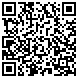
\includegraphics[width=0.25\textwidth]{reddit_thread.png}
            \caption{\url{https://www.reddit.com/r/math/comments/4d879s/most_surprising_divergent_series/}}
        \end{figure}
    \end{itemize}

\end{frame}

\begin{frame}
    \frametitle{Reddit Post — Primes with a Prime Number of Digits}

    \begin{itemize}
        \item In one example, we consider the set of prime numbers with a prime number of digits. \pause
        \item It is claimed that the sum of the reciprocals of the elements in this set diverges.
    \end{itemize} 

    \begin{figure}
        \centering
        
\includegraphics[width=0.25\textwidth]{reddit_prime_number_of_digits.png}
        \caption{\url{https://www.reddit.com/r/math/comments/4d879s/most_surprising_divergent_series/d1oppgu}}
    \end{figure}

\end{frame}

\begin{frame}
    \frametitle{Reddit Post — Numbers Without a $9$}

    \begin{itemize}
        \item In another example, we consider all of the positive integers that \emph{do not} have a $9$ \emph{anywhere} in their decimal expansion. \pause
        \item In this case, it is claimed that the sum of the reciprocals of these numbers \emph{converges}!
    \end{itemize} 

    \begin{figure}
        \centering
        
\includegraphics[width=0.25\textwidth]{reddit_kempner.png}
        \caption{\url{https://www.reddit.com/r/math/comments/4d879s/most_surprising_divergent_series/d1olh0o}}
    \end{figure}

\end{frame}

\begin{frame}
    \frametitle{Combining these Results}

    \begin{itemize}
        \item I realised that a combination of (appropriate generalisations) of these two claims implies that there are infinitely many primes which have a prime number of digits, and which contain any given string of decimal digits that you like. \pause
        \item And of course I promptly told everyone I know. \pause
        \item I even wrote a blog post about it!
        \begin{figure}
            \centering
            
\includegraphics[width=0.25\textwidth]{mathemafrica_link.png}
            \caption{\url{http://www.mathemafrica.org/?p=12942}}
        \end{figure}
    \end{itemize}
    
\end{frame}

\begin{frame}
    \frametitle{This Talk}

    \begin{itemize}
        \item In this talk, we will prove this result following the argument presented in the blog post. \pause
        \item \emph{BUT}... by considering convergent and divergent series, the blog post is needlessly circuitous. \pause
        \item It is possible to give a more direct proof of a stronger result:
        \begin{block}{Proposition}
            Given a string of digits $S$, there is some natural number $N$, such that for all $n > N$, there is a prime with $n$ digits that starts with $S$. (Or by some non-zero digit followed by $S$.)
        \end{block} \pause
        \item I will present a proof of this more general proposition towards the end of the talk.
    \end{itemize}    

\end{frame}

\section{The Harmonic and the Kempner Series}
\subsection{The Harmonic Series Diverges}
\subsection{Reciprocals of Numbers Without a Given String of Digits}

\section{Prime Numbers}
\subsection{The Prime Number Theorem}

\begin{frame}
    \frametitle{The Prime Number Theorem}

    \begin{itemize}
        \item In his talk on 1 April 2021, Lourens introduced the \emph{Prime Number Theorem}:
        \begin{theorem}[The Prime Number Theorem]
            Let $\pi(x)$ denote the number of prime numbers that are less than or equal to the real number $x$. Then
            \[
                \pi(x) \sim \frac{x}{\ln x}.    
            \]
            In other words,
            \[
                \lim_{x \to \infty} \pi(x) \Big\slash \frac{x}{\ln x} = 1.
            \]
        \end{theorem}
    \end{itemize}

\end{frame}

\begin{frame}
    \frametitle{The Prime Number Theorem}

    \begin{itemize}
        \item Formally, this means that for every $\varepsilon > 0$, there exists $N > 0$ such that
        \[
            (1 - \varepsilon) \frac{x}{\ln x} \leq \pi(x) \leq (1 + \varepsilon) \frac{x}{\ln x}    
        \]
        whenever $x > N$. \pause
        \item One consequence of this is that if $p_n$ is the $n^\text{th}$ prime number, then $p_n \sim n \ln n$. \pause
        \item Indeed, since $\pi(p_n) = n$, we have that
        \[
            \lim_{n \to \infty} \frac{p_n}{n \ln n} = \lim_{n \to \infty} \frac{\ln p_n}{\ln n} \times \frac{p_n}{\ln p_n} \Big\slash \pi(p_n).
        \]
        \item It is possible to show in an elementary way that $\lim_{n \to \infty} \ln p_n \slash \ln n = 1$, from which the result follows.
    \end{itemize} 

\end{frame}

\subsection{Reciprocals of the Primes}
\subsection{Reciprocals of Primes With a Prime Number of Digits}
\subsection{A Generalisation}

\section{Putting it All Together}

\section{A More Direct Proof}

\section{Try It Out Yourself}

\begin{frame}
    \frametitle{Website}

    \begin{itemize}
        \item I took some time to implement the Bailie-PSW pseudo-primality test in javascript. \pause
        \item This allowed me to create a site where you can enter a string of digits, and it will find up to $100$ prime numbers with a given number of digits containing the given string of digits. \pause
        \item You can try it out here:
        \begin{figure}
            \centering
            
\includegraphics[width=0.25\textwidth]{prime_strings.png}
            \caption{\url{https://dlnnlsn.github.io/prime-strings}}
        \end{figure}
    \end{itemize} 

\end{frame}

\end{document}